\documentclass{article}
\usepackage{hyperref}
\usepackage{listings}
\usepackage{color}
\usepackage{xcolor}
\usepackage{geometry}
\usepackage{graphicx}
\usepackage{amsmath}
\usepackage{caption}
\usepackage{subcaption}
\usepackage[capitalise]{cleveref}
\usepackage{wrapfig}
\usepackage{amssymb}

\geometry{margin=1in}
\pdfminorversion=6

\newcommand\TODO[1]{\textcolor{red}{TODO: #1}}

\newcommand\header[2]{
    \begin{center}
        {\large
        UCSD CSE 167 Assignment #1: \\
        \vspace{0.3cm}
        \Large
        #2}
    \end{center}
}

\definecolor{dkgreen}{rgb}{0,0.6,0}
\definecolor{gray}{rgb}{0.5,0.5,0.5}
\definecolor{mauve}{rgb}{0.58,0,0.82}
\lstset{frame=tb,
        aboveskip=3mm,
        belowskip=3mm,
        showstringspaces=false,
        columns=flexible,
        basicstyle={\small\ttfamily},
        numbers=none,
        numberstyle=\tiny\color{gray},
        keywordstyle=\color{blue},
        commentstyle=\color{dkgreen},
        stringstyle=\color{mauve},
        breaklines=true,
        breakatwhitespace=true,
        tabsize=2
}

% Taken from https://tex.stackexchange.com/questions/83085/how-to-improve-listings-display-of-json-files

\colorlet{punct}{red!60!black}
\definecolor{delim}{RGB}{20,105,176}
\colorlet{numb}{magenta!60!black}

\lstdefinelanguage{json}{
    basicstyle=\normalfont\ttfamily,
    numberstyle=\scriptsize,
    stepnumber=1,
    numbersep=8pt,
    showstringspaces=false,
    breaklines=true,
    frame=lines,
    tabsize=2,
    literate=
     *{0}{{{\color{numb}0}}}{1}
      {1}{{{\color{numb}1}}}{1}
      {2}{{{\color{numb}2}}}{1}
      {3}{{{\color{numb}3}}}{1}
      {4}{{{\color{numb}4}}}{1}
      {5}{{{\color{numb}5}}}{1}
      {6}{{{\color{numb}6}}}{1}
      {7}{{{\color{numb}7}}}{1}
      {8}{{{\color{numb}8}}}{1}
      {9}{{{\color{numb}9}}}{1}
      {:}{{{\color{punct}{:}}}}{1}
      {,}{{{\color{punct}{,}}}}{1}
      {\{}{{{\color{delim}{\{}}}}{1}
      {\}}{{{\color{delim}{\}}}}}{1}
      {[}{{{\color{delim}{[}}}}{1}
      {]}{{{\color{delim}{]}}}}{1},
}

\hypersetup{colorlinks=true}


\begin{document}

\header{4}{3D Modeling}

\begin{figure}[h]
    \centering
    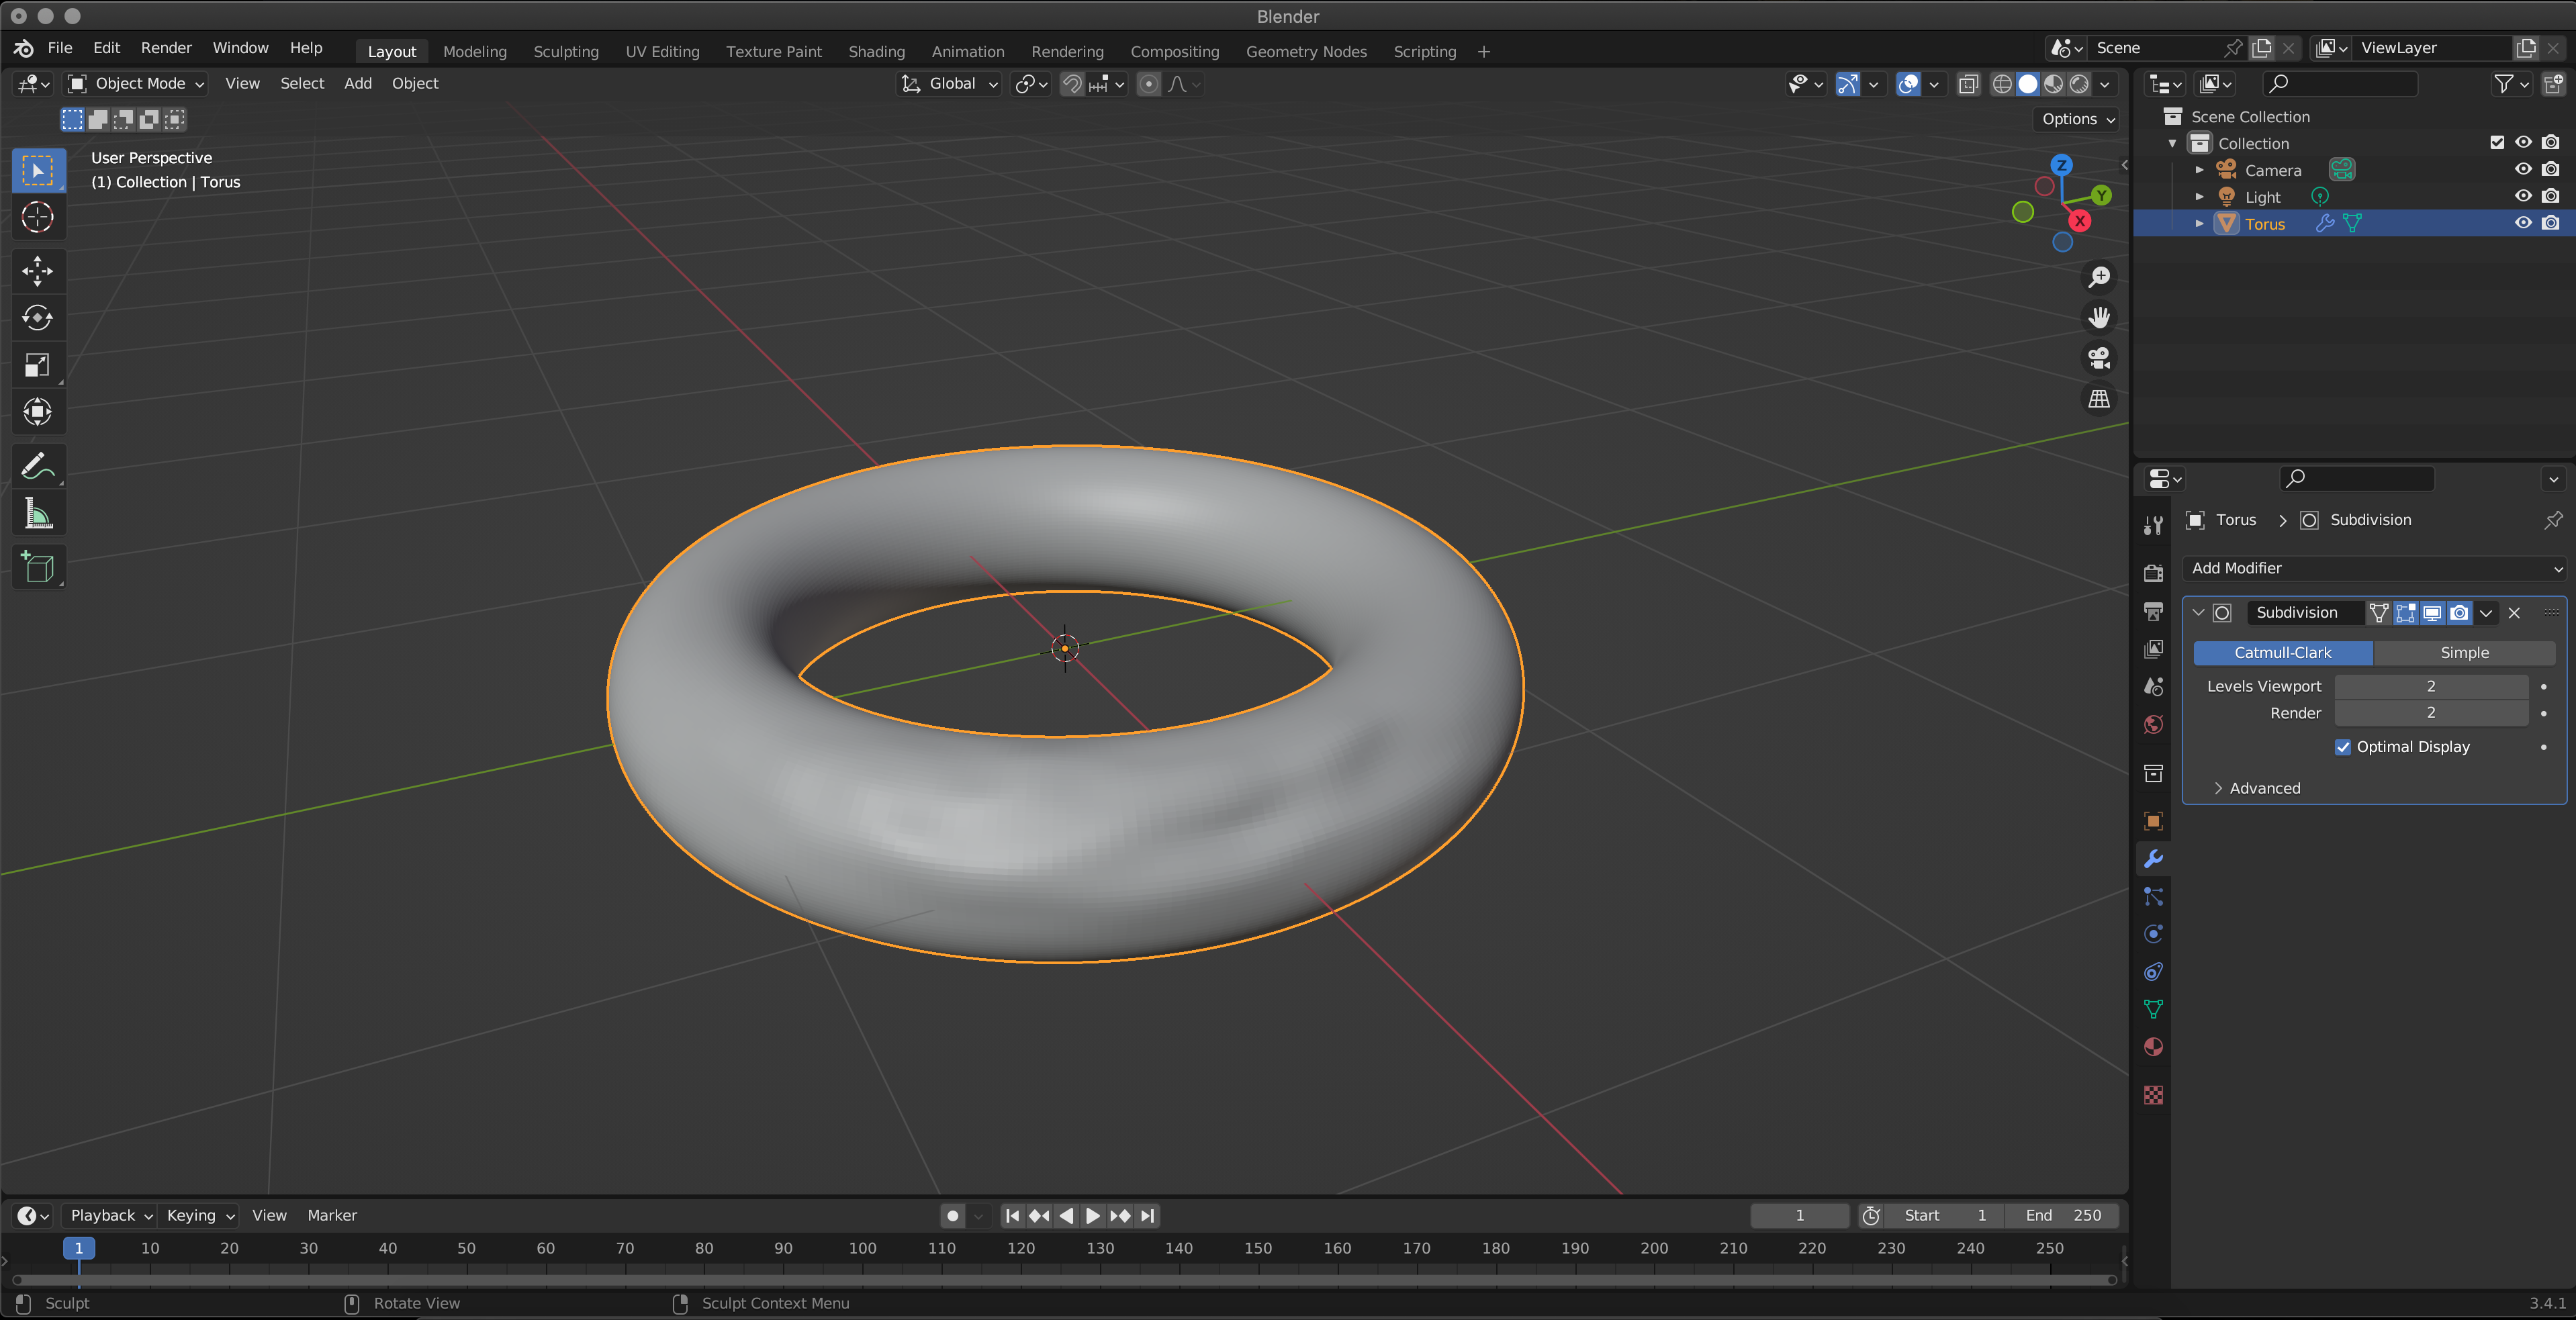
\includegraphics[width=0.5\linewidth]{imgs/hw_4.png}
    \caption{We will explore 3D modeling using Blender in this homework.}
    \label{fig:teaser}
\end{figure}

In the previous homeworks, we have provided you the models, but we didn't discuss too much about how to design new models. You can hand type triangle mesh vertices and indices, but that's not going to work when there are millions of triangles. In this homework, we will explore using a 3D modeling software to create 3D models. This homework involves significantly less programming compared to last part. The goal is to provide you a sense of how 3D models are created in general.

The 3D modeling software we will use is \href{https://www.blender.org/}{Blender}. Blender is probably the best open source and free 3D modeler for visual effects and video games. In fact it is extensively used in production (see the \href{https://www.blender.org/get-involved/user-stories/}{official blog} for a list of user stories). The commercial counterparts are \href{https://www.sidefx.com/products/houdini/}{Houdini}, \href{https://www.autodesk.com/products/maya/overview}{Maya}, \href{https://www.autodesk.com/products/3ds-max/overview}{3ds Max}. In the Computer Aided Design (CAD) industry, \href{https://en.wikipedia.org/wiki/AutoCAD}{AutoCAD}, \href{https://www.rhino3d.com/}{Rhino3D}, and \href{https://www.sketchup.com/}{SketchUp} are often used. All the 3D modeling softwares have similar features, but focus on very different design and interfaces due to the difference in applications.

For this homework, we will follow a Blender tutorial, create a 3D model, export one or more \lstinline{.ply} files, and render them using your Homework 3 renderer. We will follow the tutorial from \href{https://www.youtube.com/playlist?list=PLjEaoINr3zgEPv5y--4MKpciLaoQYZB1Z}{Blender Guru} on Youtube. I recommend watching until at least part 8 (Rendering). The tutorial will teach you how to make a donut in Blender. For the homework, we ask you to make at least two models: one that is a donut, and one that is not a donut (so that we have some diversity in the models we get!). Export them as \lstinline{.ply} files in Blender and create a \lstinline{.json} file, and render them using your Homework 3 renderer. Save a screenshot for each model as
\begin{lstlisting}[language=bash]
outputs/hw4_donut.png
outputs/hw4_not_donut.png
\end{lstlisting}
For the non-donut image, you can also make a real scene that is not just a single model, but a collection of them. Also submit your \lstinline{.ply} files and the \lstinline{.json} scene files.

We won't grade you on the quality of the resulting models. As mentioned, the purpose of this homework is simply to make you have a sense of how these models are created. As long as you make something that looks like a donut, and something that doesn't look like a donut, you're good. However, to make things more interesting, let's have a small competition for extra credits: we will post everyone's non donut image, and each person can vote for 3 of their favorite renderings. We will give 20 percent of extra credits to the top 10 winners.

\paragraph{Exporting models.} Exporting models that are compatible to our renderer is not entirely trivial since our renderer does not support all features in Blender. Firstly, to export your Blender model/scene to a \lstinline{.ply} file, click \lstinline{File} and then click \lstinline{Export}, and you will see the option of exporting your scene to a \lstinline{.ply} file (make sure to select \emph{Triangulated Mesh} in the options). However, this will only export the geometry, and will not export the textures/colors you assigned to the surface. For those, we will need to use the ``Bake'' feature in Blender Cycles. Before you bake, first change the material of your model from Principled BSDF to Diffuse. To bake the colors to an image texture or vertex colors, first go to the Render Properties tab in the Properties panel (by default it's on the right). Next, change the Render Engine in the tab to Cycles. Next, go to Bake and change the Bake Type to Diffuse, and remove checks on Direct/Indirect Contributions in Influence. For baking to an image texture, set the Output Target to Image Textures. For baking to vertex colors, choose Active Color Attribute for the Output Target. Click Bake to bake the color to the textures or vertex colors. For the vertex colors, you need to have an active color attribute for the baking to work -- the easiest way to achieve this is to switch to the Vertex Paint mode (by default it's on the top left), and paint something on your model. You can also directly use the Vertex Paint to create the desired vertex color.

\end{document}
